
\documentclass{l4proj}

%Packages
\usepackage{natbib}

\begin{document}
\title{Augmented Reality Android Gym App}
\author{David Benicek 2073063b}
\date{\today}
\maketitle

\begin{abstract}
Something will go here.
\end{abstract}

\educationalconsent
%
%NOTE: if you include the educationalconsent (above) and your project is graded an A then
%      it may be entered in the CS Hall of Fame
%
\tableofcontents
%==============================================================================

\chapter{Introduction}
\pagenumbering{arabic}
\section{Motivation}
Frequent exercise and a healthy lifestyle have recently become an integral part of the western culture. Indeed, last year in America more people have exercised on a regular basis then ever before \cite{USexercise}. As people begin to adopt this new and healthy lifestyle it is immediately obvious that there are two distinct periods during which there seems to be a lack of coherent information. These are at the very beginning when a person begins to exercise for the first time and when a person begins to plateau and starts to experience diminishing returns for their work due to a lack of variation in their routine. It is important to note that a lack of coherent information does not necessarily mean a lack of data but instead a lack of a singular consensus in the midst of conflicting information, fad diets, ill-informed advice and 'bro science'. It therefore, seems that there is a need for a singular portal to which both beginners and experienced gym goers alike can refer to for information regarding exercise.  

\section{Aim} \label{sec:aim}
Tackling the entire topic of fitness in one application would be extremely difficult, if not impossible. Due to this we are going to narrow down the focus and seek to add value to users while they are in the gym. The aim of the application will be to help users understand how to use gym equipment, suggest a range of exercises that can be carried out on a given piece of equipment and demonstrate how to perform the exercise with correct and safe form. 

One of the main goals of the app is for it to be responsive to the user's environment and heavily interactive so that the user has an immersive experience. An immersive experience will keep users engaged with the app however there is a balance to be drawn here. We must be careful as to not allow users to loose track of their surroundings completely since the gym is a potentially dangerous environment. One possible way of striking this balance is through augmented reality (AR). AR would allow us to give a somewhat immersive experience by super imposing realistic human models on their device's screen without the need for a completely virtualized reality. Similar applications of AR have been trialed in education, construction, sports and medicine to various degrees of success. A review of literature regarding previous work done with AR can be found in section \ref{sec:litrew}.

\section{Outline}
In this document we are going to explore the different steps taken in the development of the augmented reality gym app. First, we will review relevant literature in order to be able to make informed decisions concerning requirements and constraints. Requirements elicited from discussions with the Glasgow University Sports Association  and any other partys will also be review and summarized. Following, will be a discussion of the possible designs of the app from both a user experience and user interface aspect. Later we will go trough the steps in implementation and testing, outlining the procedure and any major problems along the way. Finally, we will draw the document to a close with a conclusion, followed by an evaluation where we will address to what extend the main goals of the project were achieved and reflect on what could have been done differently for future reference. 

\chapter{Requirements}


\section{Review of previous work} \label{sec:litrew}
The term 'augmented reality' was coined by a Boeing researcher, Tom Caudell in 1990\nocite{rauterberg_history_2002}. Since then, AR has been used in a number of disciplines ranging from medicine to entertainment or construction.\nocite{azuma_recent_2001} (TODO: page 3-9). It seems that there has been no previous research done into the possible application of AR in the fitness sector and therefore we will draw on insights from previous pedagogical applications of AR with the hope of drawing parallels between pedagogical teaching and instructing users to perform exercises in the gym. 

Squire and Klopfer identified the shrinking of technologies from desktop to mobile as a key opportunity for AR simulation to migrate over to handheld devices and carried out teaching experiments with AR which yieleded largely positive results \nocite{squire_augmented_2007}. AR allowed students the opportunity to explore "phenomena impossible to produce in the real world, such as diseases or toxic chemical" leaks \nocite{squire_augmented_2007} (TODO: page 372). One of the main advantages of AR is that the user needn't imagine the locational context of the situation since they are actually in it and can thus better understand and learn the information being conveyed. This is supported by the idea of situativity as proposed by Greeno which argues that immersing oneself in the context of a situation aids with its understanding\nocite{greeno_situativity_1998}. By developing a mobile application which is to be used in a gym, we will be able to exploit the idea of situativity and have an advantage over desktop systems and applications.

(TODO tie this in somehowwwww)
Radu has also entertained the application of AR in education and found that there are numberous benefits\nocite{radu_why_2012}. In this experiment AR increased understanding and long-term retention of content and also improved student motivation\nocite{radu_why_2012}. Each of these are very important factors both for students and for gym goers. Improved understanding and retention of information could distinguish an AR gym application from other non-AR applications. Furthermore, if users find themselves more motivated thanks to using the AR gym application, this would be a significant selling point.

There are however also some issues with AR. Usability difficulties and fluctuating levels of understanding between students have been registered when AR is used as an educational tool \nocite{radu_why_2012} and therefore usability and heuristics of the app will need to be at the center of attention. One of the main issues is allignment \nocite{sood_pro_2012}. Object recognition, especially on mobile devices, does not yet have the needed fidelity to be able to distinguish the same object in different variations. For example, object recognition could be used to recognize a bench in the gym however it will only ever be able to recognize that specific type of bench. In a different gym, with different benches or even with the same bench but different lighting, shadows and perhaps colour, object recognition will do us no good. One possible solution, proposed by Rekimoto and Ayatsuka is to have visual tags on the objects and use these to identify them \nocite{rekimoto_cybercode:_2000}. We can group objects that are the same or similar by giving them the save tag and placing it in the correct area. We then use object recognition to recognize the tag and use it as an anchor for our augmented reality overlay. By tracking the position and size of the visual tag we can move and size our augmentation accordingly. 

Perhaps the most important issue when creating a phone app in general and an AR app in particular is the issue of attention tunneling \nocite{radu_why_2012} \nocite{biocca_attention_2007}. Using AR is a relatively immersive experience and we must therefore take care to highlight appropriate things to the user. We want to find a balance between focusing on the app and focusing on the world around the user. Biocca et al. have pointed out that attention funneling is a problem with mobile interfaces in general, stating that "the attention demands of current interfaces such as cellular phones and PDAs may play a significant role in automobile accidents". Some AR applications such as Pokemon Go have solved the issue of attention tunneling through pop ups that remind the user to stay aware of their surroundings \nocite{hollister_drivers_2016}. A similar approach should be adopted in our application to ensure the users safety and must be one of the high priority requirements.

On the topic of safety, the demonstrated exercises could pose a health and safety risk to the users. There are often many different ways to carry out a single exercise and frequently there is no consensus on the best approach. Most of the times there will be an ideal motor pattern to lift the most weight efficiently, in theory, however when a user tries to recreate this, they might be put in a compromising position. Take, for example, the deadlift (picking up a bar from the floor and finishing in a standing position with the bar mid thigh). Within the app we may demonstrate that the safest starting position is from a half-squat where the thighs make a 25° angle with the floor. This may indeed be the safest position for someone with a perfectly proportionate body, but if somebody has shorter arms and longer legs, they may need to squad down further to reach the bar and be in a strong position. If such a user were to follow our instructions too closely they may round their back too much in order to reach down to the bar and end up hurting themselves. If a user was so inclined, they could blame the app for providing unsafe instructions to them. One possible solution to this problem is by having a disclaimer either as a pop up within the app or on the loading screen. If a user is clearly made aware that the demonstrated form for each exercise is only approximate and shows what the creators deemed most efficient, then there should be no liability issues. 

\subsection{Meeting with GUSA}
When developing an app of any kind it is important to consider how you are going to market and distribute the finished product. This question is particularly interesting in our context because the app needs some real-life components (markers) to work and therefore needs to be pitched to both daily users and gyms. One of the first steps that I carried out, before doing much research into technologies and development was to arrange a meeting with the Glasgow University Sports Association (GUSA). I pitched my idea to the president of GUSA in an email and was able to arrange a meeting both with GUSA president and the Sport Development Manager at Glasgow University. The meeting 	was held on the 26th of July 2016 and yielded a number of interesting requirements and points of discussion, many of which I had not previously considered. 

One point of discussion was the issue of liability. The main goal of the app is to demonstrate what perfect form of an exercise looks like, however there are conflicting views as to what 'perfect' form for an exercise is. One expert might argue one way and another might be completely opposed which will mean that the app will have to choose a side. If the chosen side is eventually found to be incorrect, or worse, dangerous there could be options of liability. A potential solution would be to show a disclaimer on or during app launch that notifies the user that all demonstrations of form are approximate and that the user should contact an expert if they are unsure how to properly and safely perform an exercise. 

GUSA was cautious about how the app is going to be distributed and marketed since they are themselfs working on a designated GUSA app and are also pushing the LifeFitness app to their customers. The main concern was that by having too many apps marketed in the gym, customers would be overwhelmed and end up using none of the apps. It was decided that in order to solve this dilemma, my app would not be distributed by GUSA nor will it have any relation to GUSA. Instead the Glasgow university gym will simply be an environment for testing. 


\chapter{Design}
\section{User Experience}
The quick brown fox jumped over the lazy dog.
The quick brown fox jumped over the lazy dog.
The quick brown fox jumped over the lazy dog.
The quick brown fox jumped over the lazy dog.
\section{User Interface}
The quick brown fox jumped over the lazy dog.
The quick brown fox jumped over the lazy dog.
The quick brown fox jumped over the lazy dog.
The quick brown fox jumped over the lazy dog.

\chapter{Implementation}
The development of an augment reality phone application sounds quite daunting at first. The image recognition, 3D object imaging and use of sensors and mathematical calculations to pivot the projected image are undoubtedly complex however luckily for us, there are many libraries and tools that allow us to abstract the complex intricate work and allow us to focus on the core app development. Having said that, the initial learning curve to find, set up and get started with all the tools and technologies is quite steep. In this section we are first going to explore the numerous tools used throughout the project, justify their selection and talk about how they are used. Later we will talk about some of the challenges that had to be overcome during the implementation process.
\subsection{Technologies used}
\subsubsection{Git}
One of the first tools that was set up as a part of the project was the Git version control system. Git is usually used in the open source community or within teams to allow easy integration between contributors however in our case Git is used to keep a backup of old versions of the project and to share the progress of the project with the project supervisor. 

\subsubsection{Vuforia}
Vuforia is one of the many open source augmented reality libraries \cite{vuforia}. Vuforia provides an online interface where you can upload different images which are then analysed for specific feature patterns that are used for matching. For example figure \ref{fig:coca_cola_features} show the feature patterns of a CocaCola logo. A collection of such targets can be exported as a database and later used in Unity for matching using optical recognition \cite{vuforia_unity}.
\begin{figure}
\centering

\includegraphics[scale=1]{images/coca_cola_features.png}
\caption{Patterns of features on the CocaCola logo.}
\label{fig:coca_cola_features}
\end{figure}

Vuforia allows us to create markers but it is also a plugin for Unity and an SDK that is used in native Android code development \cite{vuforia_unity}.

\subsubsection{Unity}


\subsubsection{MakeHuman}


\subsection{Trials and Tribulations }
 
\chapter{Testing}

\chapter{Conclusion}

\chapter{Evaluation}

%\vspace{-7mm}
\begin{figure}
\centering
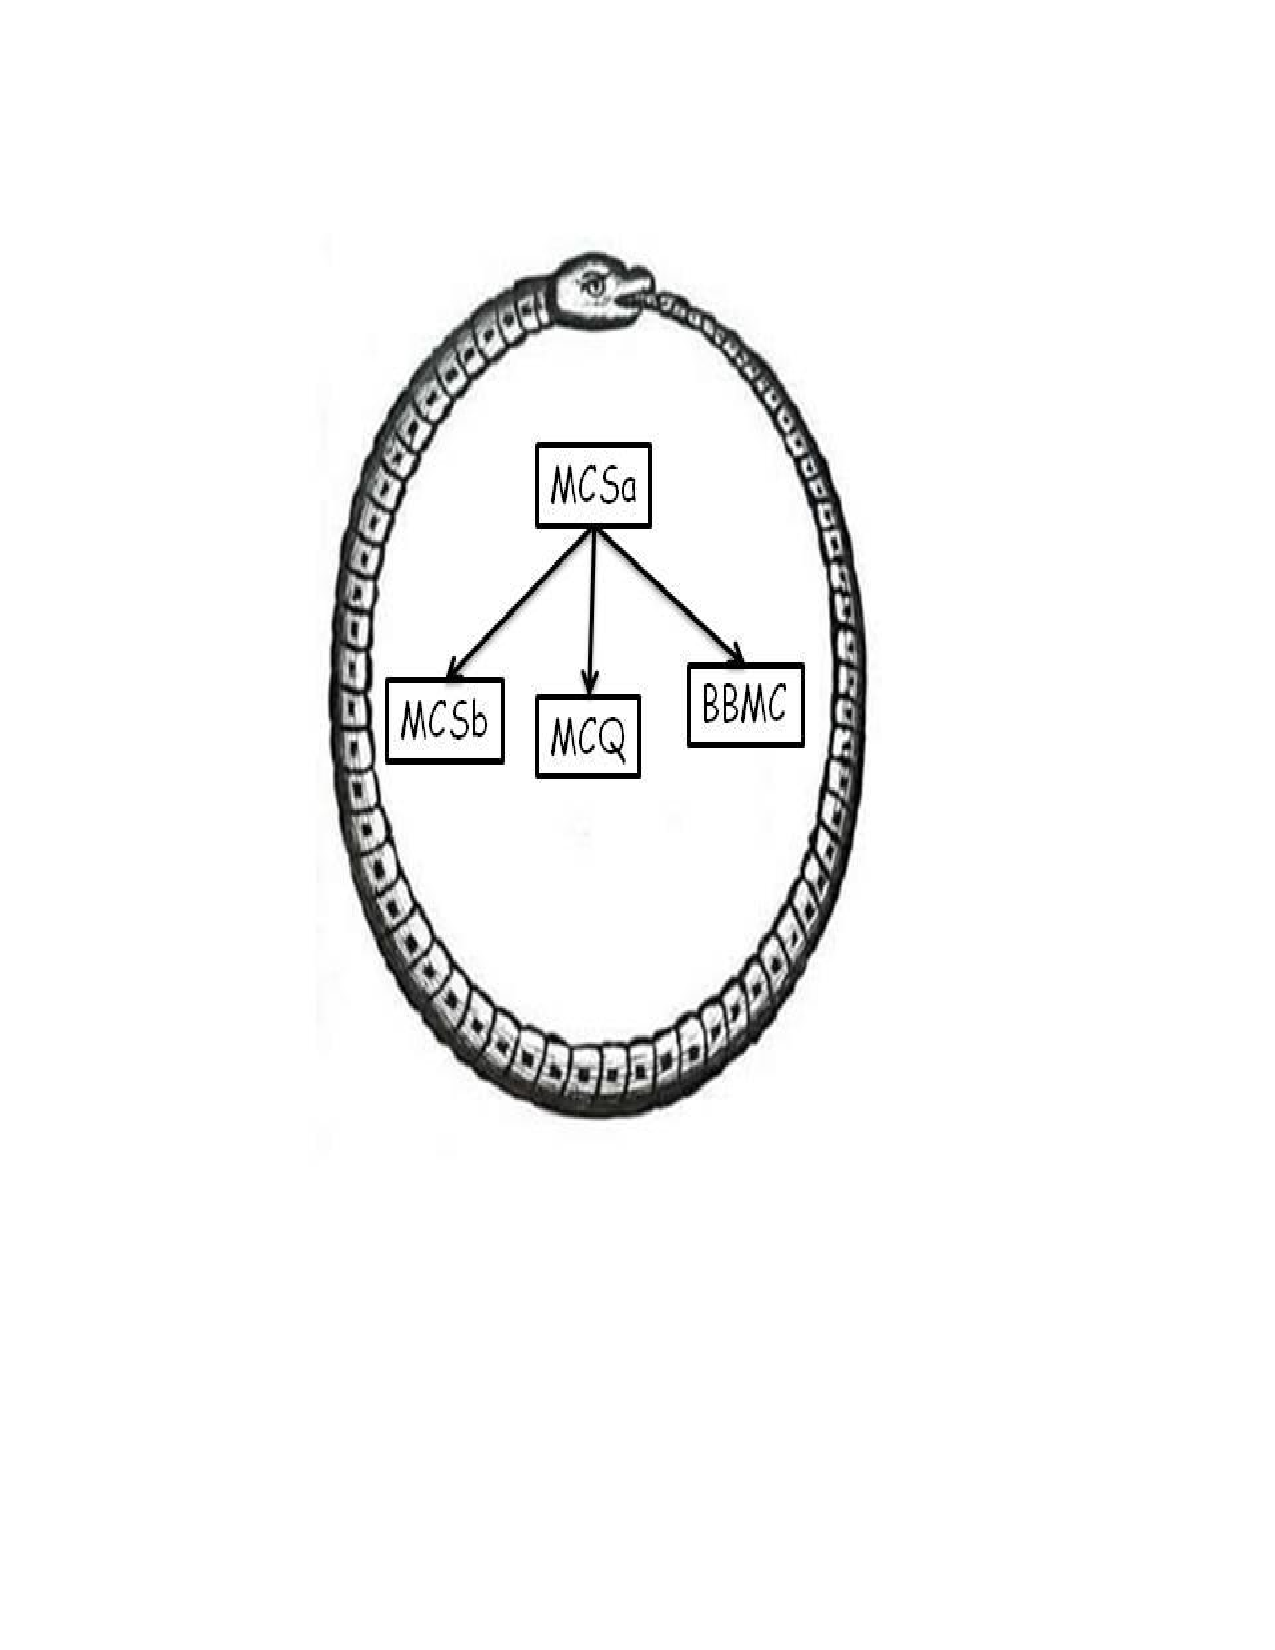
\includegraphics[height=9.2cm,width=13.2cm]{uroboros.pdf}
\vspace{-30mm}
\caption{An alternative hierarchy of the algorithms.}
\label{uroborus}
\end{figure}



%%%%%%%%%%%%%%%%
%              %
%  APPENDICES  %
%              %
%%%%%%%%%%%%%%%%
\begin{appendices}

\chapter{Running the Programs}
An example of running from the command line is as follows:
\begin{verbatim}
      > java MaxClique BBMC1 brock200_1.clq 14400
\end{verbatim}
This will apply $BBMC$ with $style = 1$ to the first brock200 DIMACS instance allowing 14400 seconds of cpu time.

\chapter{Generating Random Graphs}
\label{sec:randomGraph}
We generate Erd\'{o}s-R\"{e}nyi random graphs $G(n,p)$ where $n$ is the number of vertices and
each edge is included in the graph with probability $p$ independent from every other edge. It produces
a random graph in DIMACS format with vertices numbered 1 to $n$ inclusive. It can be run from the command line as follows to produce 
a clq file
\begin{verbatim}
      > java RandomGraph 100 0.9 > 100-90-00.clq
\end{verbatim}
\end{appendices}

%%%%%%%%%%%%%%%%%%%%
%   BIBLIOGRAPHY   %
%%%%%%%%%%%%%%%%%%%%

\bibliographystyle{plain}
\bibliography{bib}

\end{document}
